%\documentclass{scrartcl}
\documentclass{standalone}
\usepackage{tikz,ifthen}
\usetikzlibrary{math}

%
% Customize colors
%
\definecolor{chapter-color}{cmyk}{1, 0.50, 0, 0.25}
\definecolor{link-color}{cmyk}{1, 0.50, 0, 0.25}
\definecolor{cite-color}{cmyk}{0, 0.7, 0.9, 0.2}
\definecolor{codegreen}{rgb}{0,0.6,0}
\definecolor{codegray}{rgb}{0.5,0.5,0.5}
\definecolor{codepurple}{rgb}{0.58,0,0.82}
\definecolor{backcolour}{rgb}{0.95,0.95,0.92}
\definecolor{codebgcolor}{RGB}{129, 139, 152}
\definecolor{codehighlightcolor}{RGB}{255, 230, 153}
%\definecolor{codegreen}{RGB}{0, 153, 0}
%\definecolor{codegray}{RGB}{127, 127, 127}
\definecolor{codeblue}{RGB}{102, 214, 237}
\definecolor{codekeyword}{RGB}{249, 36, 114}
\definecolor{codecomment}{RGB}{127, 127, 127}
\definecolor{backcolor}{RGB}{242, 242, 235}
\definecolor{linkcolor}{RGB}{102, 0, 0}
\definecolor{corange}{RGB}{255, 70, 0}
\definecolor{cyellow}{RGB}{209, 153, 0}
\definecolor{cblue}{RGB}{64, 128, 255}
\definecolor{cbrown}{RGB}{153, 102, 51}
\definecolor{cpink}{RGB}{255, 0, 255}
\definecolor{cred}{RGB}{255, 64, 0}
\definecolor{cgreen}{RGB}{0, 191, 0}
\definecolor{clightblue}{RGB}{191, 217, 255}
\definecolor{cturquois}{RGB}{0, 255, 255}
\definecolor{cpurple}{RGB}{128, 0, 255}
\definecolor{clightgreen}{RGB}{175, 255, 175}
\definecolor{clightgray}{RGB}{211, 211, 211}
\definecolor{clightpink}{RGB}{255, 175, 255}
\definecolor{cdarkblue}{RGB}{0, 0, 255}
\definecolor{cdarkred}{RGB}{255, 0, 0}
\definecolor{cdarkgreen}{RGB}{0, 255, 0}
\definecolor{cgray}{RGB}{153, 153, 153}

\definecolor{myblue}{RGB}{55, 126, 184}
\definecolor{myorange}{RGB}{255, 127, 0}
\definecolor{myred}{RGB}{228, 26, 28}
\definecolor{mypurple}{RGB}{152, 78, 163}
\definecolor{mygreen}{RGB}{77, 175, 74}
\definecolor{myyellow}{RGB}{255, 255, 51}
\definecolor{mybrown}{RGB}{166, 86, 40}
\definecolor{mypink}{RGB}{166, 86, 40}
\definecolor{mygray}{RGB}{153, 153, 153}


\begin{document}
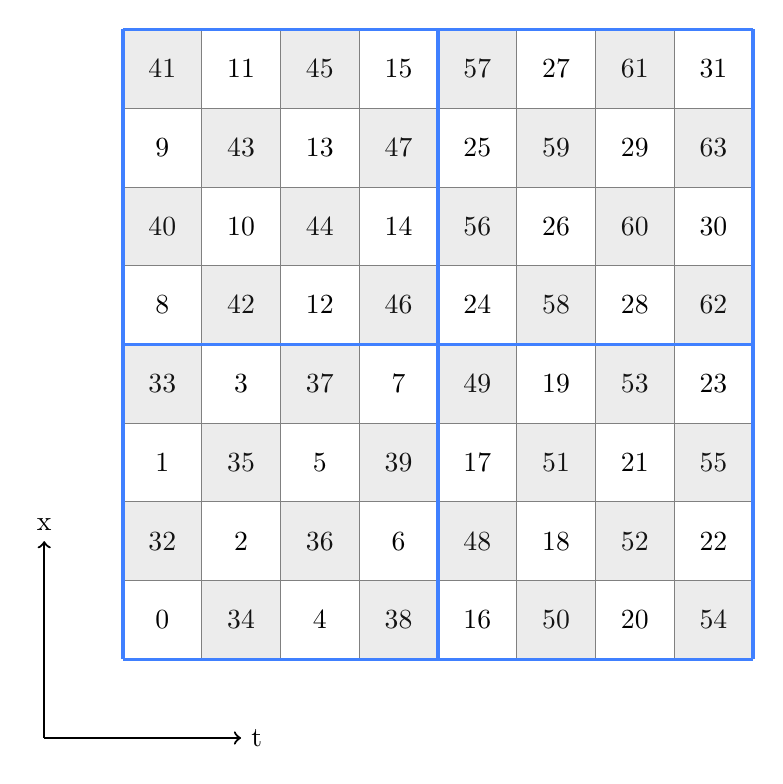
\begin{tikzpicture}

\tikzmath{
% first cache block
let \evenoffset = 0;
let \oddoffset = 32;
let \offset = (0.5, 0.5);
int \ix;
for \x in {0,1,...,3}{
  for \y in {0,1,...,3}{
    \ix = (4*\x + \y)/2 + \evenoffset;
    if Mod(\x+\y,2) == 1 then {
        \ix = \ix + \oddoffset;
    };
    {
      \draw \offset + (\x,\y) node{\ix};
    };
  };
};
% second cache block
let \evenoffset = 8;
let \offset = (0.5, 4.5);
int \ix;
for \x in {0,1,...,3}{
  for \y in {0,1,...,3}{
    \ix = (4*\x + \y)/2 + \evenoffset;
    if Mod(\x+\y,2) == 1 then {
        \ix = \ix + \oddoffset;
    };
    {
      \draw \offset + (\x,\y) node{\ix};
    };
  };
};
% third cache block
let \evenoffset = 16;
let \offset = (4.5, 0.5);
int \ix;
for \x in {0,1,...,3}{
  for \y in {0,1,...,3}{
    \ix = (4*\x + \y)/2 + \evenoffset;
    if Mod(\x+\y,2) == 1 then {
        \ix = \ix + \oddoffset;
    };
    {
      \draw \offset + (\x,\y) node{\ix};
    };
  };
};
% fourth cache block
let \evenoffset = 24;
let \offset = (4.5, 4.5);
int \ix;
for \x in {0,1,...,3}{
  for \y in {0,1,...,3}{
    \ix = (4*\x + \y)/2 + \evenoffset;
    if Mod(\x+\y,2) == 1 then {
        \ix = \ix + \oddoffset;
    };
    {
        \draw \offset + (\x,\y) node{\ix};
    };
  };
};
% checkerboard coloring
for \x in {0,1,...,7}{
  for \y in {0,1,...,7}{
    if Mod(\x+\y,2) == 1 then {
        { \fill[gray,opacity=0.15] (\x,\y) rectangle ++(1,1); };
    };
  };
};
};

\draw [step=1.0,gray, very thin] (0,0) grid (8,8);
\draw [step=4.0,cblue, very thick] (0,0) grid (8,8);

\draw[thick,->] (-1,-1) -- (1.5,-1) node[right]{t};
\draw[thick,->] (-1,-1) -- (-1,1.5) node[above]{x};

\end{tikzpicture}
\end{document}
